% Created 2020-09-30 Wed 15:22
% Intended LaTeX compiler: pdflatex
\documentclass[10pt,t]{beamer}
\usepackage[utf8]{inputenc}
\usepackage[T1]{fontenc}
\usepackage{graphicx}
\usepackage{grffile}
\usepackage{longtable}
\usepackage{wrapfig}
\usepackage{rotating}
\usepackage{amsmath}
\usepackage{textcomp}
\usepackage{amssymb}
\usepackage{capt-of}
\usepackage{hyperref}
\usetheme{default}
\author{L. Larrabee Strow}
\date{\today}
\title{\large AIRS Cloud Fraction Trends from a PDF-based Approach Compared to PATMOS}
\subtitle{\footnotesize{AIRS Virtual Science Team Meeting}}
\date{\vspace{0.1in}\footnotesize{May 12, 2019 \vfill}}
\author{L. Larrabee Strow\inst{1,2}, Andy Tangborn \inst{2}, and Howard Motteler\inst{2} }
\institute[UMBC]{\inst{1} UMBC Physics Dept. \and \inst{2}UMBC JCET}
\input beamer_setup
\usetheme{metropolis}
\metroset{titleformat title=allcaps}
\renewcommand{\UrlFont}{\small\tt}
\renewcommand*{\UrlFont}{\footnotesize}
\tolerance=1000
\begin{document}

\maketitle

\begin{frame}[label={sec:org80ad0c8}]{No graphics, one block}
\begin{block}{Patmosx}
\begin{itemize}
\item Heidinger A. et. al., The Pathfinder Atmospheres–Extended AVHRR Climate Dataset, V 95  BAMS, 2014
\item Starts in 1983
\item AVHRR based, very high spatial resolution
\item Many cloud products, not just cloud fraction
\item Fairly heavily used, long-term NOAA support
\end{itemize}

Patmosx has been used for climate model studies, more below.   \\

Validation versus AIRS L3 and/or MODIS could follow\ldots{}
\end{block}
\end{frame}

\begin{frame}[label={sec:org6169a6e}]{One graph}
Grid point in Atlantic Ocean south of northern Africa: at (-5,0)\textdegree{} lat/lon, (1.8,3.0)\textdegree{}

\begin{center}
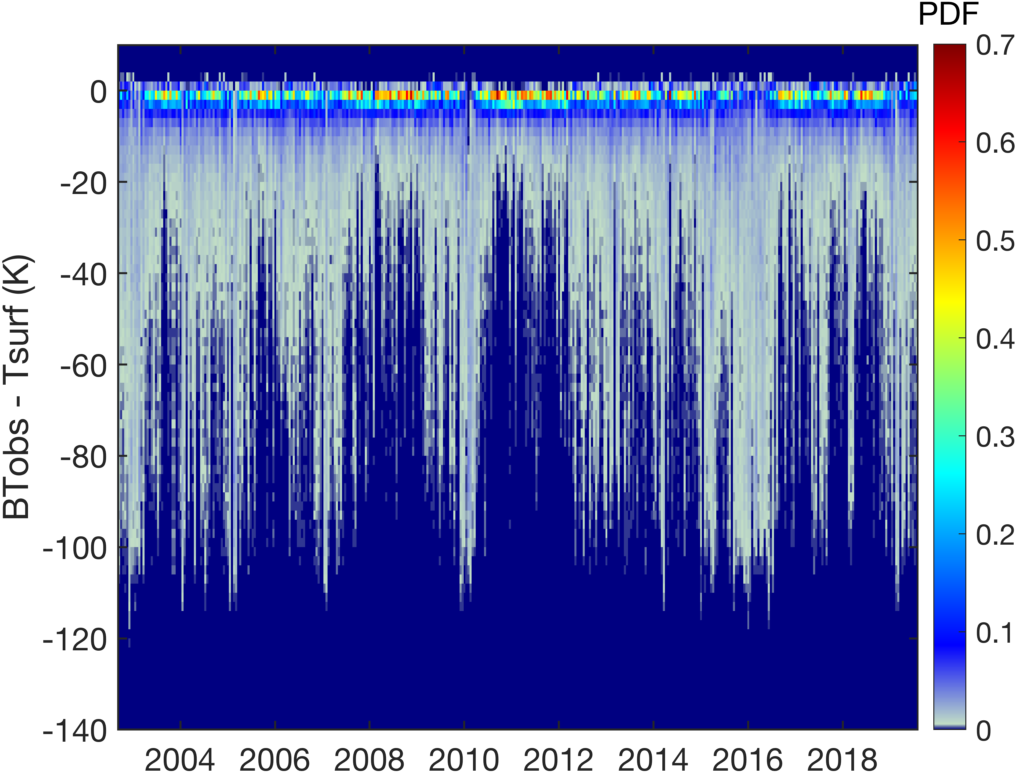
\includegraphics[width=0.8\linewidth]{./Figs/airs_pdf_bin_0long_m5deglat_windchan.png}
\end{center}
\end{frame}

\begin{frame}[label={sec:org409cb32}]{4 graphs, bottom two have block titles}
\vspace{-0.6in}
\begin{columns}
\begin{column}{0.55\columnwidth}
\begin{block}{}
\begin{center}
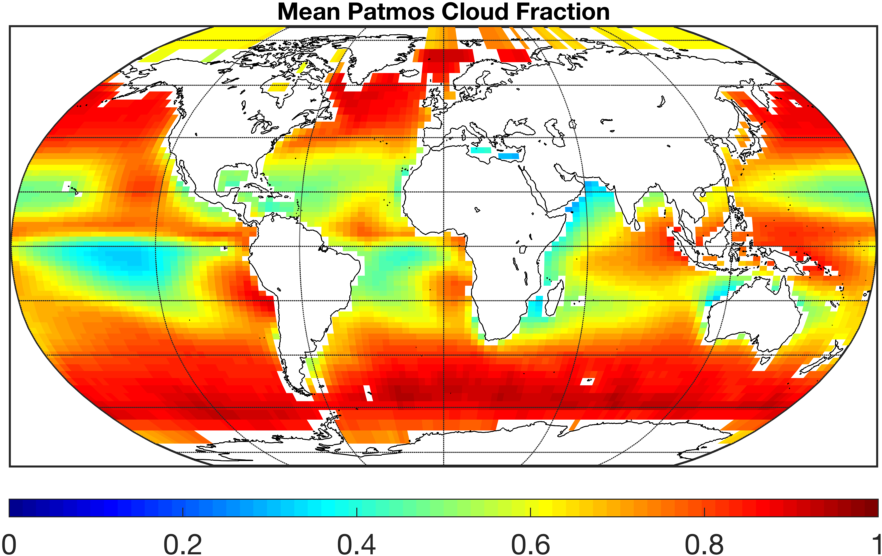
\includegraphics[width=\linewidth]{./Figs/patmos_mean_cloud_frac.png}
\end{center}
\end{block}
\end{column}

\begin{column}{0.55\columnwidth}
\begin{block}{}
\begin{center}
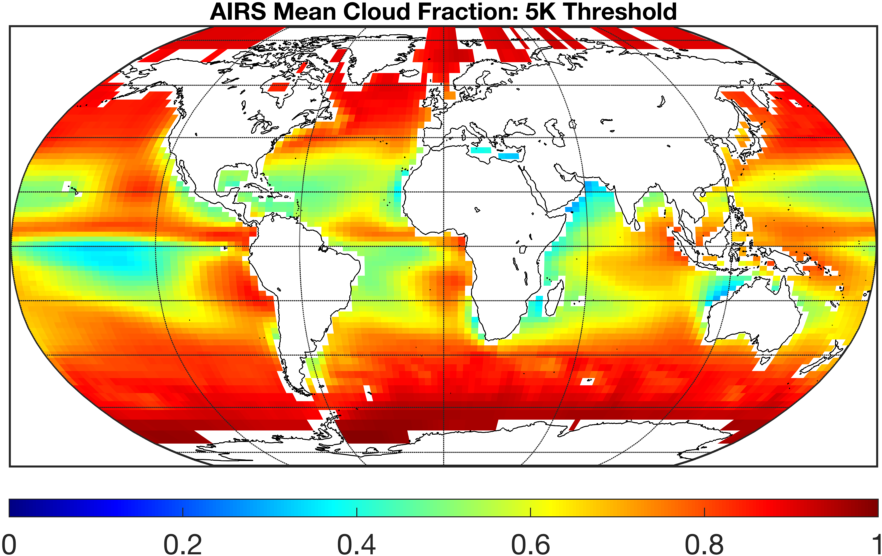
\includegraphics[width=\linewidth]{./Figs/airs_mean_cloud_frac_true5K_threshold.png}
\end{center}
\end{block}
\end{column}
\end{columns}

\vspace{-0.2in}

\begin{columns}
\begin{column}{0.55\columnwidth}
\begin{block}{\footnotesize Threshold = 5K}
\vspace{-0.1in}

\begin{center}
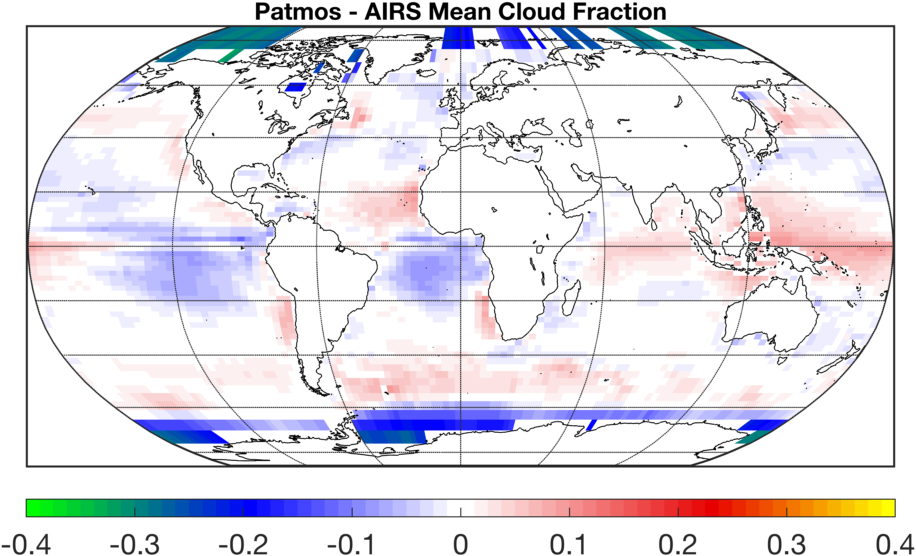
\includegraphics[width=\linewidth]{./Figs/patmos_minus_airs_mean_cloud_frac_true5Kcloud.png}
\end{center}
\end{block}
\end{column}

\begin{column}{0.55\columnwidth}
\begin{block}{\footnotesize Threshold = 10K}
\vspace{-0.1in}

\begin{center}
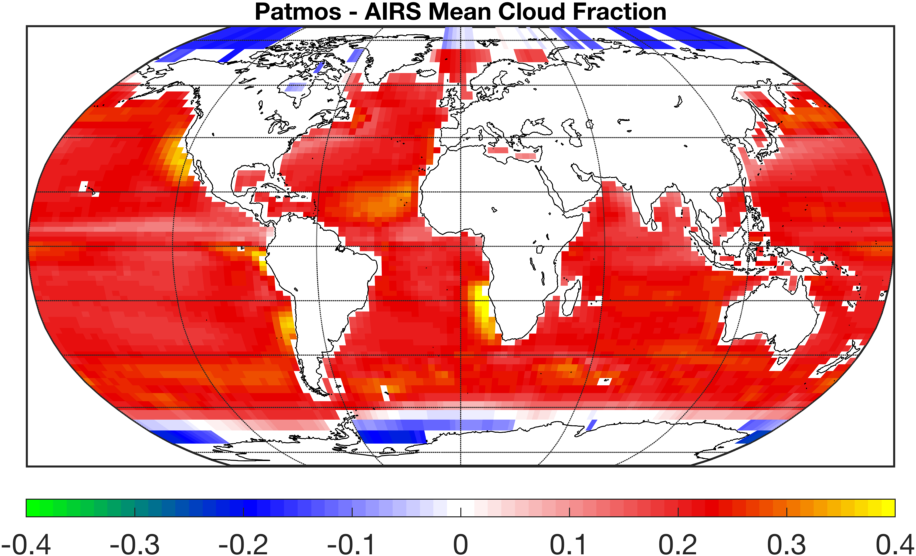
\includegraphics[width=\linewidth]{./Figs/patmos_minus_airs_mean_cloud_frac.png}
\end{center}
\end{block}
\end{column}
\end{columns}
\end{frame}

\begin{frame}[label={sec:orgffcde70}]{One graph, two column blocks below}
\vspace{-0.15in}

\begin{center}
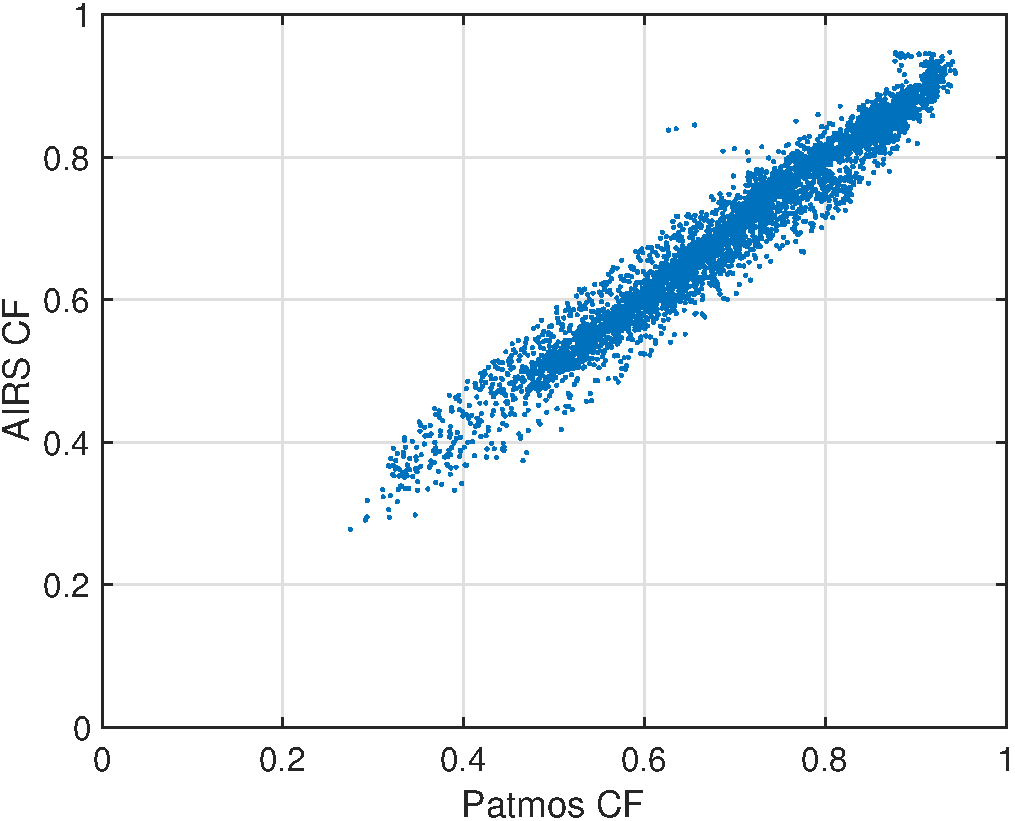
\includegraphics[width=0.55\linewidth]{./Figs/scatter_cloud_airs_patmos_pm60lat_threshold5p5.pdf}
\end{center}

\vspace{-0.3in}

\begin{columns}
\begin{column}{0.6\columnwidth}
\begin{block}{Cloud Fraction}
\begin{footnotesize}
\begin{itemize}
\item Correlation Coefficient:  0.98
\item Mean (Patmos - AIRS):  0.37\% \textpm{} 2.5\% (std)
\item Mean (Patmos - AIRS): \textpm{}60\textdegree{} lat= 0.03\% \textpm{} 3\% (std)
\end{itemize}
\end{footnotesize}
\end{block}
\end{column}
\begin{column}{0.6\columnwidth}
\begin{block}{Cloud Trends}
\begin{footnotesize}
\begin{itemize}
\item Mean (Patmos - AIRS): -0.05 \textpm{}0.12 \%/yr (std)
\item Mean (Patmos - AIRS): \textpm{}60\textdegree{} lat = = -0.066 \textpm{}0.015 \%/yr (std)
\end{itemize}
\end{footnotesize}
\end{block}
\end{column}
\end{columns}

\vspace{-0.05in}
\footnotesize Estimated AIRS trend uncertainty due to SST trend errors:  \textasciitilde{}0.06\%/yr 2\(\sigma\)
\end{frame}

\begin{frame}[label={sec:org6e6f3d0}]{Two graphs side-by-side}
\begin{itemize}
\item Many similarities, but note Equatorial Atlantic
\item Note SAO issue for Patmosx
\item Note scale is cloud fraction in \%
\end{itemize}

\begin{columns}
\begin{column}{0.55\columnwidth}
\begin{block}{}
\begin{center}
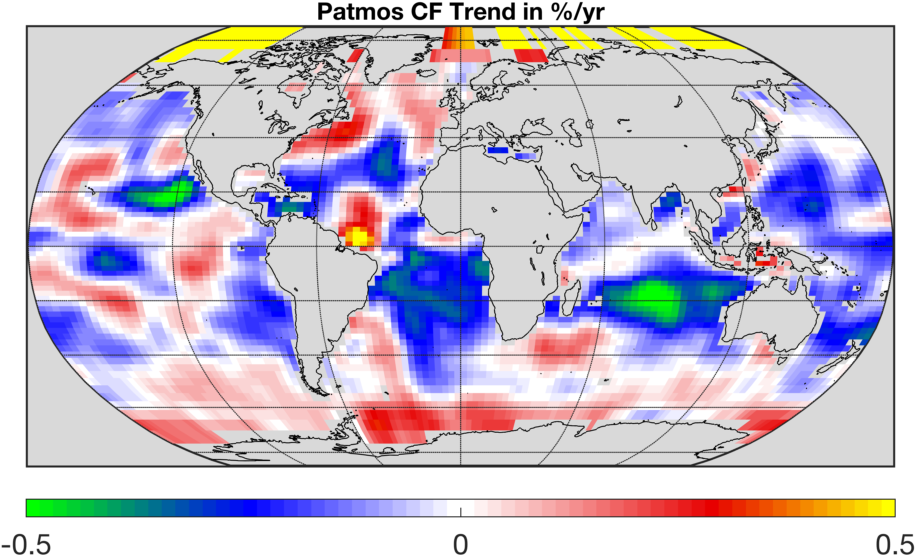
\includegraphics[width=\linewidth]{./Figs/patmos_cf_rate_smooth.png}
\end{center}
\end{block}
\end{column}


\begin{column}{0.55\columnwidth}
\begin{block}{}
\begin{center}
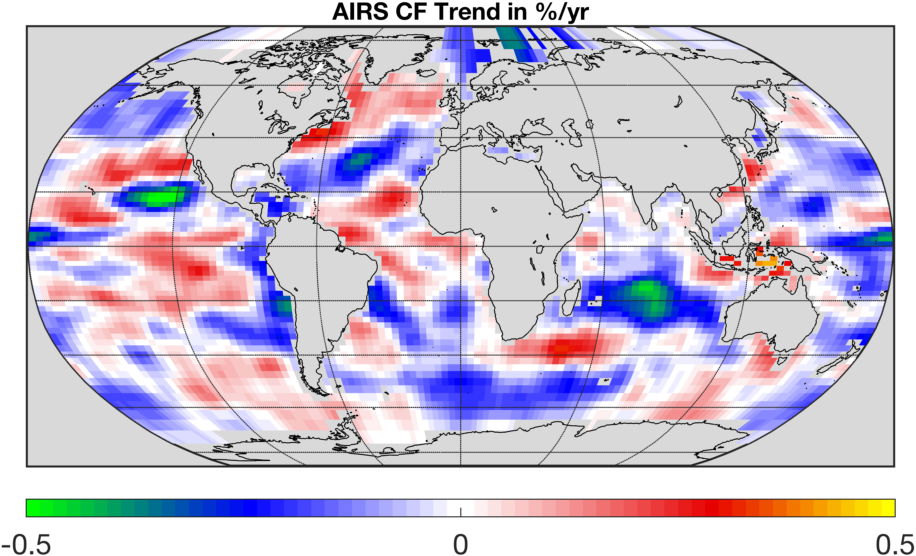
\includegraphics[width=\linewidth]{./Figs/airs_cf_rate_smooth.png}
\end{center}
\end{block}
\end{column}
\end{columns}
\end{frame}

\begin{frame}[label={sec:org3c4166f}]{2x2 (4 graphs), no headers, use this a lot}
\vspace{-0.5in}
\begin{columns}
\begin{column}{0.55\columnwidth}
\begin{block}{}
\begin{center}
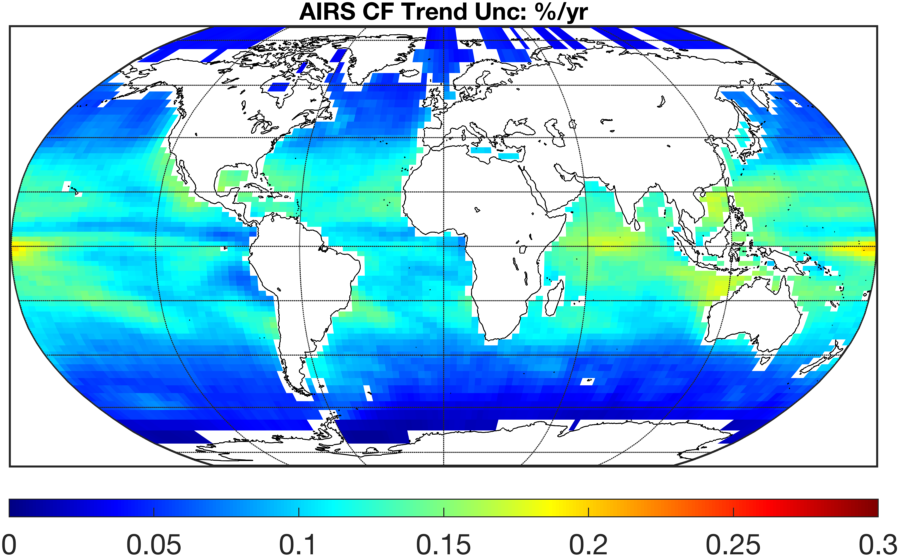
\includegraphics[width=\linewidth]{./Figs/airs_percent_trend_unc.png}
\end{center}
\end{block}
\end{column}

\begin{column}{0.55\columnwidth}
\begin{block}{}
\begin{center}
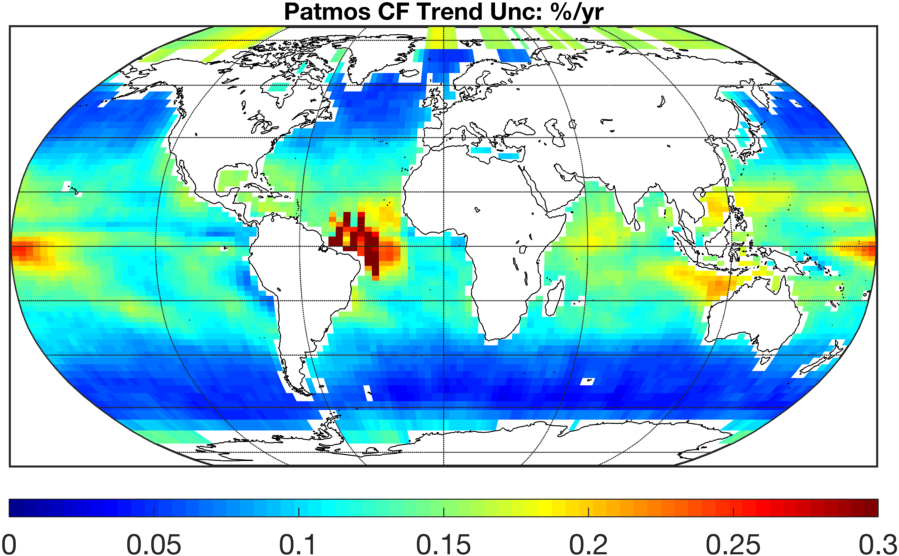
\includegraphics[width=\linewidth]{./Figs/patmos_percent_trend_unc.png}
\end{center}
\end{block}
\end{column}
\end{columns}

\vspace{-0.45in}
\begin{columns}
\begin{column}{0.55\columnwidth}
\begin{block}{}
\begin{center}
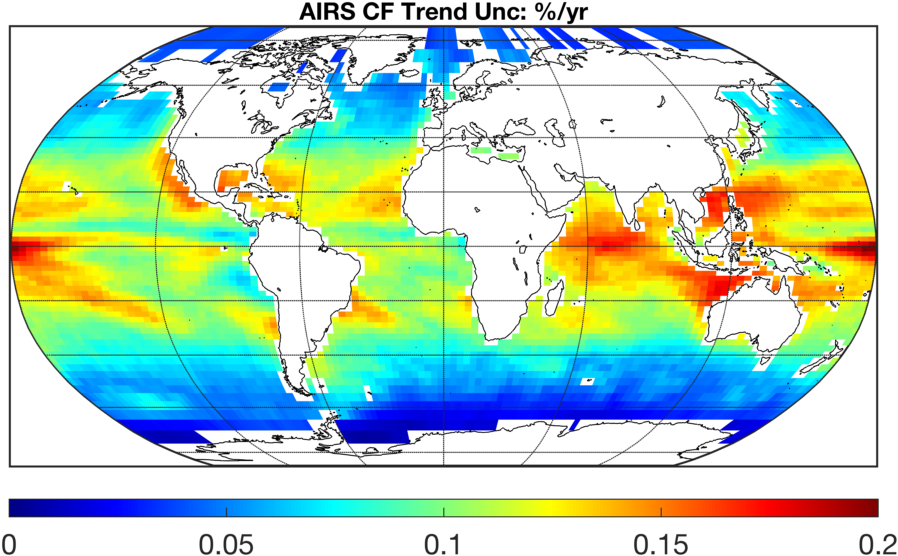
\includegraphics[width=\linewidth]{./Figs/airs_percent_trend_unc_czoom.png}
\end{center}
\end{block}
\end{column}
\begin{column}{0.55\columnwidth}
\begin{block}{}
\begin{center}
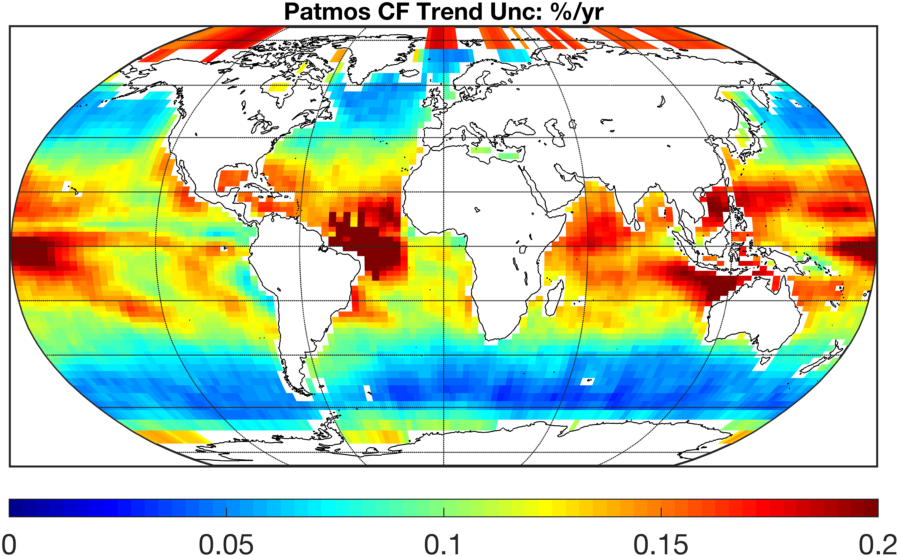
\includegraphics[width=\linewidth]{./Figs/patmos_percent_trend_unc_czoom.png}
\end{center}
\end{block}
\end{column}
\end{columns}
\end{frame}
\end{document}